\chapter{Methodology}
\label{ch:Methodology}
This chapter outlines the technical methodology adopted in the development of the system, covering both low-level design and software implementation. The approach prioritizes performance, privacy, and modularity, leveraging hardware accelerators where possible and maintaining efficient control over data flow and execution.


%----------------------
%----------------------
\section{Application Modules and Design}
\label{sec:ApplicationDesignModules}
%----------------------

This section provides an overview of the internal architecture and design principles behind the TLDR desktop application. The application is built with the goal of providing a fast, private, and efficient interface for question-answering and summarization tasks over a user-defined corpus of documents. To achieve this, the design incorporates several performance-aware and hardware-conscious modules, especially tailored for Apple’s M1/M2 architecture.

The TLDR system is structured into modular components, each responsible for a specific functionality in the information processing pipeline. These include embedding generation, context retrieval, vector storage, prompt construction, and output generation via a language model. The workflow between these modules is coordinated to support seamless execution, low latency, and high responsiveness, all while maintaining data privacy by running entirely on-device.


%----------------------
\subsection{Overview}
\label{subsec:AppDesignModules-Overview}
%----------------------
The TLDR application follows a modular architecture where different components are responsible for distinct tasks in the RAG (Retrieval-Augmented Generation) pipeline. Figure~\ref{fig:tldr_modules} illustrates the overall design and the control flow between the modules.

\begin{figure}[H]
    \centering
    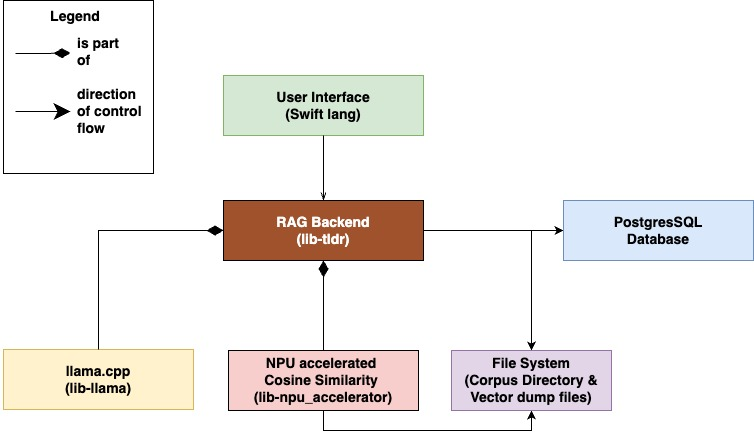
\includegraphics[width=1.0\linewidth]{images/tldr-app-modules.jpg}
    \caption{Modules of TLDR application}
    \label{fig:tldr_modules}
\end{figure}


\begin{itemize}
    \item \textbf{User Interface:} This module provides the graphical frontend for the user. Developed using Swift language for MacOS, it allows users for the users to seamlessly leverage the capabilities of the application. It is responsible for workflows dealing with user experience while delegating all core logic to the backend modules.

    \item \textbf{RAG Backend:} This is the core orchestrator of the application. It manages the full pipeline, including handling user queries, initiating vector search, performing retrieval, and forwarding context to the language model. It communicates with all supporting modules such as the database, NPU based vector search module, llama.cpp and the file system.

    \item \textbf{Database (PostgreSQL):} Stores metadata and document indexing information. It ensures efficient retrieval and persistence of preprocessed documents and vector references. It is plays a crucial role of mapping retrieved vector hashes to their text chunks and document metadata during context retrieval.

    \item \textbf{File System (Corpus Directory and Vector Dump Files):} Contains the document corpus (directory containing source documents) and their corresponding vector dump files. These vector dump are leveraged by the vector search engine using memory-mapped I/O for efficient vector search with low memory overhead.

    \item \textbf{NPU Accelerated Cosine Similarity:} Implements hardware-accelerated cosine similarity by leveraging Apple's Neural Processing Unit (NPU). The backend invokes this module for fast and parallelizable vector cosine similarity computation.

    \item \textbf{llama.cpp:} This module is responsible for language generation i.e LLM inference. It acts as a plugged-in module for the RAG backend and contributes by generating embeddings and chat response during the corresponding stages of the RAG pipeline.
\end{itemize}


%----------------------
\subsection{User Interface}
\label{subsec:AppDesignModules-UI}
%----------------------

The User Interface is in the form of a native MacOS desktop application developed using Swift lang in the Xcode development environment (as depicted in Fig~\ref{fig:tldrGUI}, Fig~\ref{fig:tldrdockicon}). The user interface is designed to be intuitive, lightweight, and self-contained. The application packages all necessary dependencies, including static libraries and LLM weights. enabling fully offline functionality without requiring additional installation or configuration.

The user interface module has the following core purposes:
\begin{itemize}
    \item Provides a clean, chat-style interface where user prompts and LLM responses are displayed as distinct messages to mimic a conversational flow.
    \item Manager all responsibilities regarding user interaction, including persisting user conversation history and any additional user preferences and thereby enable RAG backend to only focus on the RAG functionalities.
    \item \textit{Make a single, self contained portable package that is easy and intuitive to distribute.}
\end{itemize}
\begin{figure}[H]
    \centering
    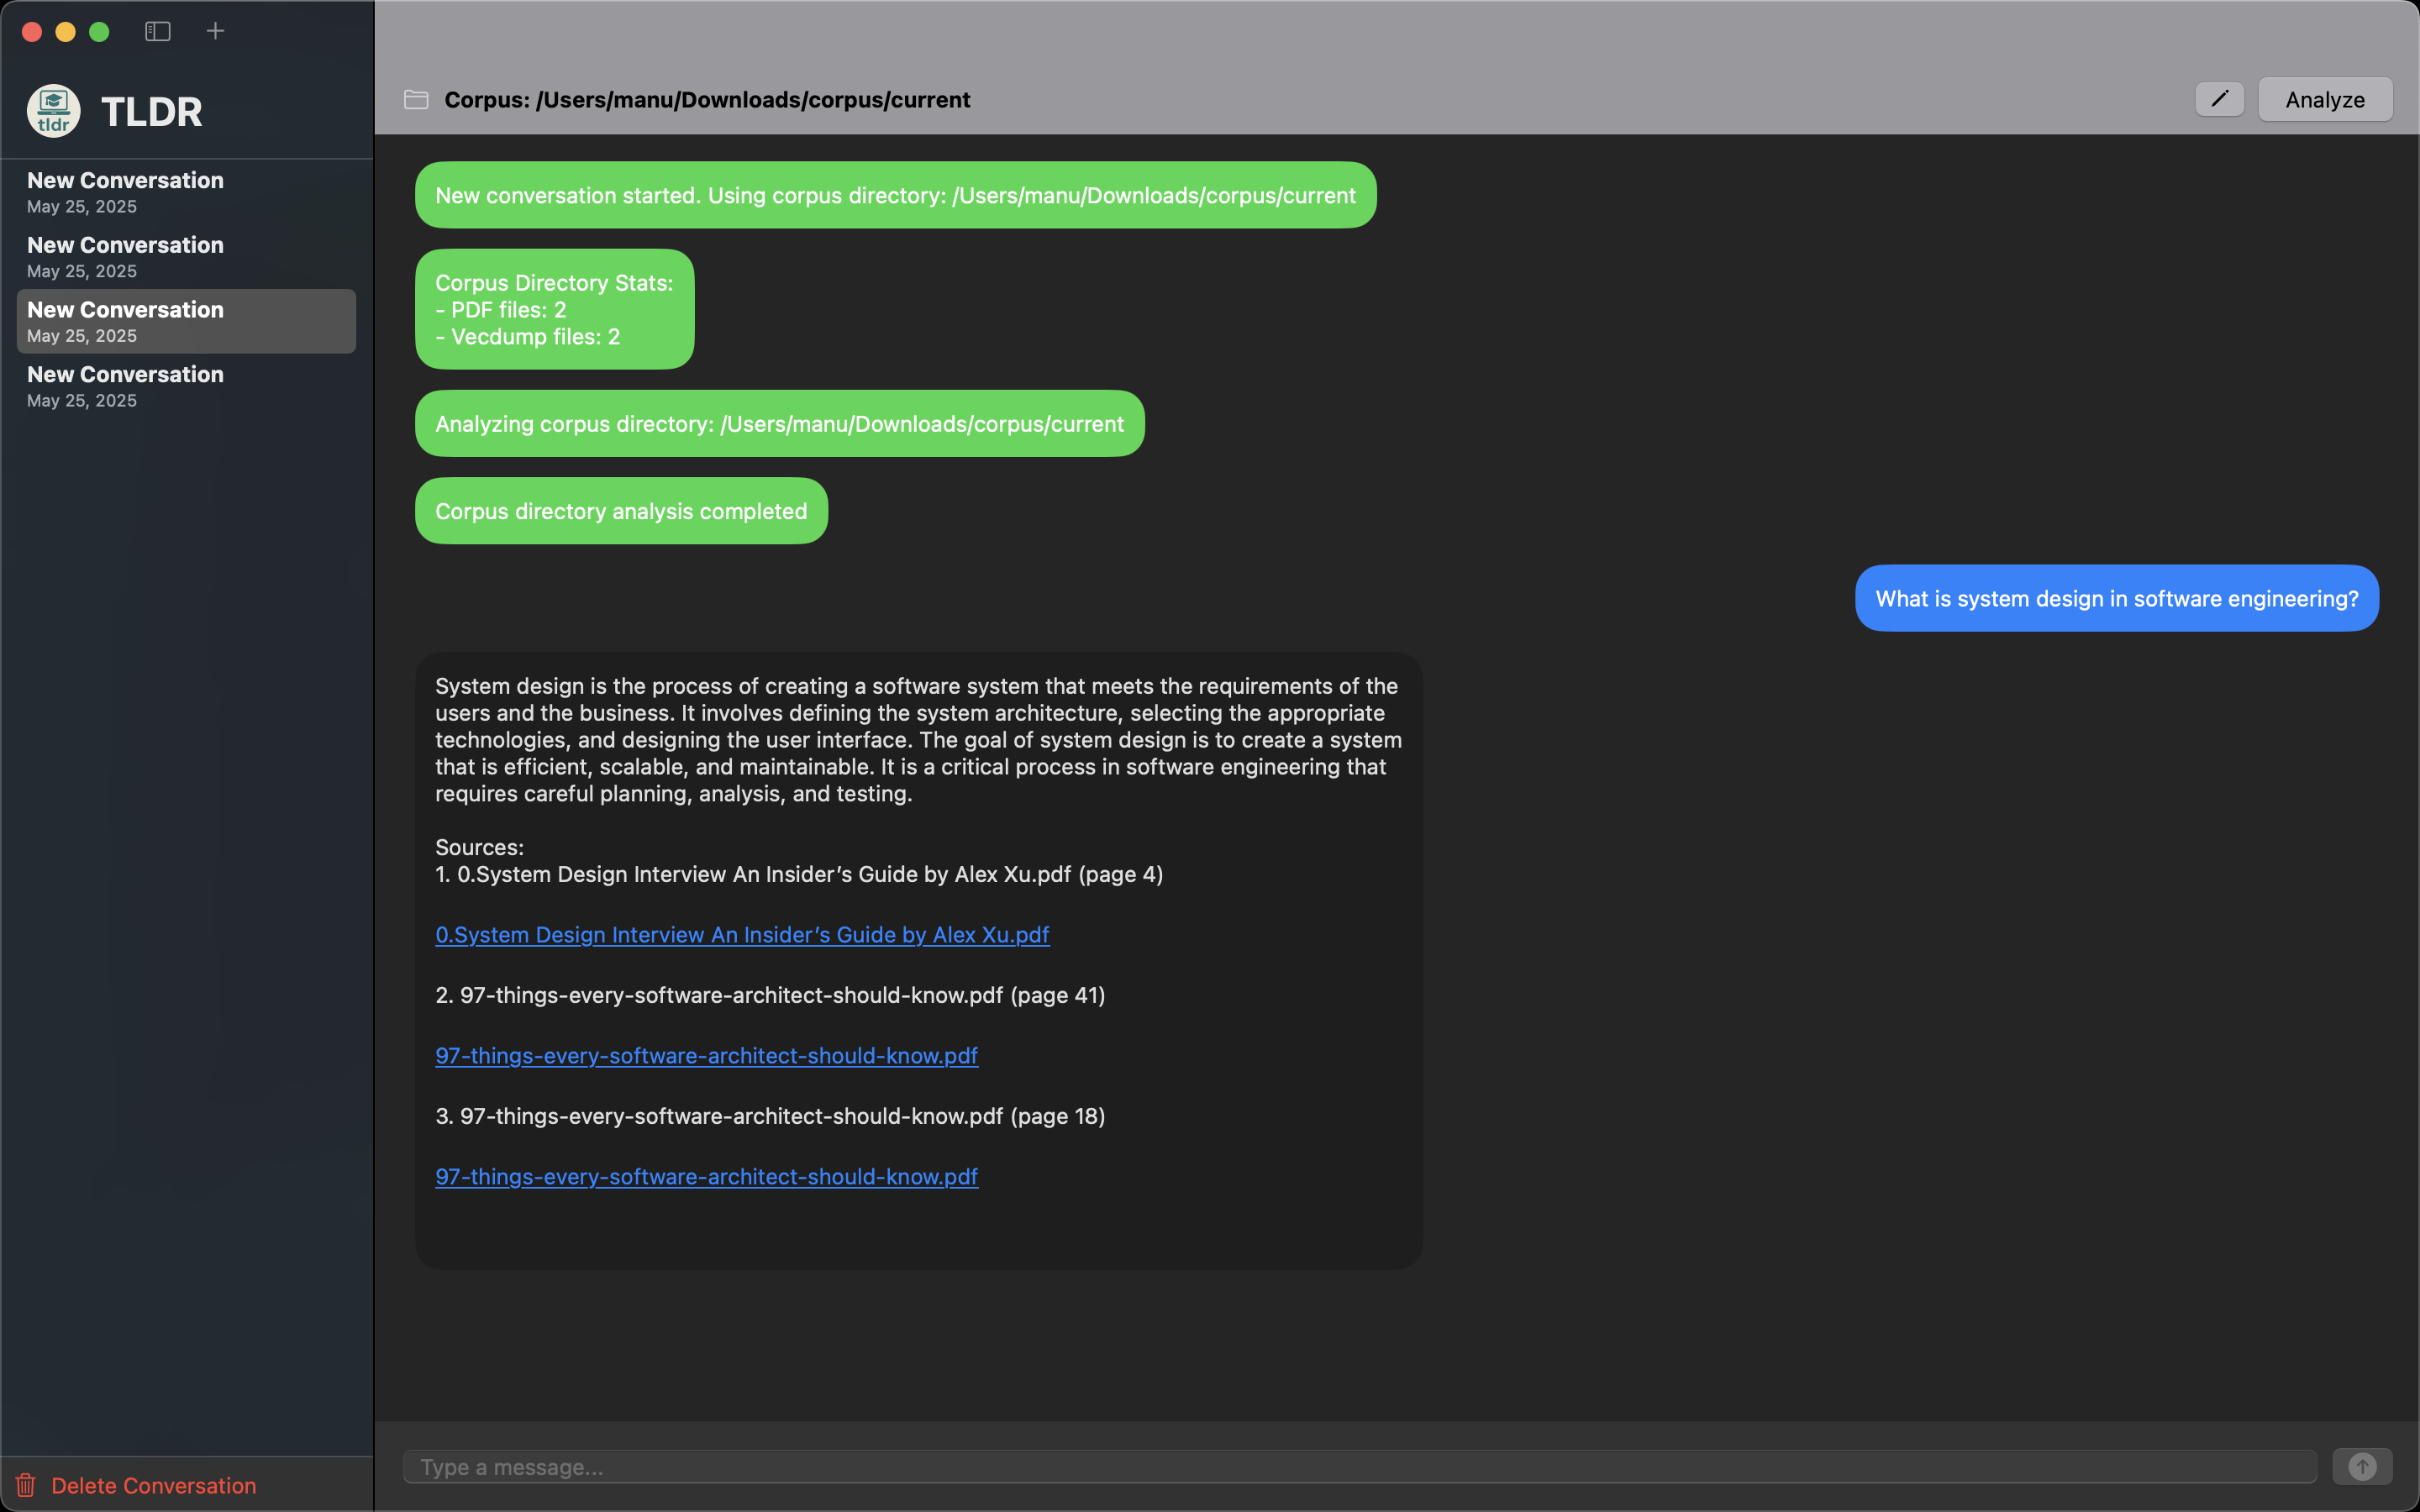
\includegraphics[width=1.0\linewidth]{images/tldr-ui-window.png}
    \caption{Graphical User Interface of TLDR Application}
    \label{fig:tldrGUI}
\end{figure}
\begin{figure}[H]
    \centering
    
\includegraphics[width=0.65\linewidth]{images/tldr-dock-icon.png}
    \caption{TLDR Application Icon as seen in MacOS Dock}
    \label{fig:tldrdockicon}
\end{figure}
%----------------------
\subsubsection{Codebase Organization}
\label{subsubsec:AppDesignModules-UICodebase}
%----------------------

The codebase of the GUI application is illustrated in Figure~\ref{fig:tldrUIFs}. It is organized into several components that serve both core functionality and supporting roles within the application. 
\begin{figure}[H]
    \centering
    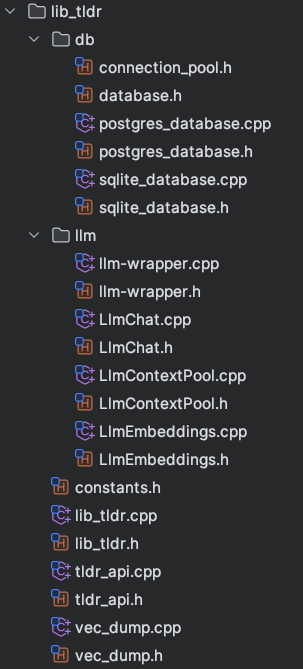
\includegraphics[width=0.5\linewidth]{images/ui-proj-fs.png}
    \caption{UI Project File system}
    \label{fig:tldrUIFs}
\end{figure}
\begin{enumerate}[label=\Alph*.]
    \item Overall Structure:
    \begin{enumerate}[label=\alph*.]
        \item \texttt{tldr}: The Swift language codebase that creates the user interface.
        \item \texttt{TldrAPI}: C++ module with bindings for Swift UI. It serves as a bridge between the Swift UI and the C++ static library of the RAG Backend.
    \item \texttt{artefacts}: Quantized LLM weights and coreml packages, i.e:
    \begin{itemize}
        \item \texttt{Llama-3.2-1B-Instruct-Q3\_K\_L} model for chat
        \item \texttt{all-MiniLM-L6-v2-Q8\_0} model for generating embeddings
        \item \texttt{CosineSimilarityBatched} coreml package for cosine similarity on NPU
    \end{itemize}
    \end{enumerate}

    \item UI Architecture (MVVM):
    \begin{enumerate}[label=\alph*.]
        \item \texttt{tldrApp}: The main SwiftUI entry point where the application lifecycle begins.
        \item Models: Includes \texttt{ConversationData}, \texttt{Message}, and \texttt{RagResultSw} to represent the chat state and RAG outputs. These modules leverage \textit{UserDefaults} a built-in key-value persistance mechanism provided by Apple's Foundation framework to efficiently store and retrieve their information.
        \item Views: Comprises SwiftUI components like \texttt{ChatView} and \texttt{ContentView} to render the main interface.
        \item ViewModels: Contains \texttt{ChatViewModel}, which handles user interaction and backend coordination.
        \item Preview Content: Includes \texttt{Preview Assets} for SwiftUI previews to support development and layout testing.
        \item Assets: Stores static resources such as icons and other UI elements.
    \end{enumerate}
\end{enumerate}
This organization promotes maintainability and allows for a clear separation of concerns between UI presentation, interaction logic, and backend communication.
%----------------------
\subsection{RAG Backend}
\label{subsec:AppDesignModules-RAG Backend}
%----------------------
\begin{figure}[htbp]
  \centering
  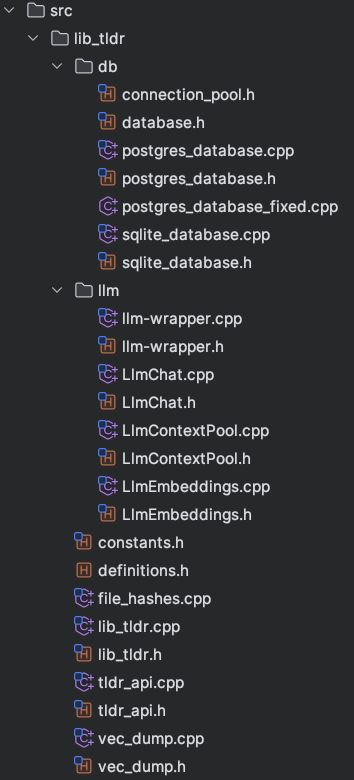
\includegraphics[width=0.5\linewidth]{images/lib_tldr_fs.png}
  \caption{RAG Backend(lib\_tldr) codebase}
  \label{fig:libTldrCodebase}
\end{figure}

The RAG backend is implemented as a C++ static library named \texttt{lib\_tldr}. It serves as the backbone for all core functionalities of the project. This module encapsulates the complete RAG pipeline logic and integrates essential components such as the large language model for text and embedding generation, the vector dump generator and reader, database and file system handlers for storage, and the cosine similarity-based vector retriever (as seen in Fig~\ref{fig:libTldrCodebase}).

The architecture emphasizes modularity and resource efficiency, enabling plug-and-play replacement or extension of components. It adheres to the SOLID principles of object-oriented programming, promoting adaptability, maintainability, and scalability.



Following are the logical sub-modules of RAG Backend:
\begin{enumerate}[label=\Alph*.]
\item{Language Model Interface:}

The system utilizes \texttt{llama.cpp} as the backend for both text generation and embedding extraction. The following components facilitate this integration:

\begin{enumerate}
    \item \texttt{LlmChat.cpp \&.h}: Manage the logic to take user input and retrieved context and generate a response from the chat LLM. 
    \item \texttt{LlmEmbeddings.cpp \&.h}: These modules extract dense vector representations (embeddings) from document chunks, which are subsequently used for semantic similarity search and retrieval.
    \item \texttt{LlmContextPool.cpp \&.h}: These components manage the lifecycle of LLM context objects, which encapsulate the model state necessary for efficient inference. Since LLMs typically require a context to maintain internal buffers, tokenizer state, and memory allocations, it is computationally expensive to initialize a new context for every query or embedding operation. By pooling and reusing contexts across multiple operations, the system significantly reduces initialization overhead and ensures smoother, low-latency performance during both chat and embedding workflows.
    \item \texttt{Llm-Wrappers.cpp \&.h}: Takes care of initializing and cleaning up resources related to the LLMs. It initializes common ggml backend for Apple metal and setting up LLM context pools and initialize Chat and Embedding LLMs by loading their weights into memory.
\end{enumerate}

\item{Database Interaction:}
All persistent storage is handled via the PostgreSQL backend, though an optional SQLite backend is also implemented (but not currently utilized). The database interaction is managed within the \texttt{db} submodule, which includes the following:

\begin{enumerate}[label=\alph*.]
\item \texttt{database.h}\: Defines an abstract class that enforces a uniform interface for any underlying database implementation. This design allows the RAG codebase to remain unchanged when switching between different database technologies.
    \item \texttt{postgres\_database.cpp \&.h}: These files handle database initialization, schema definition, and CRUD operations related to documents and embeddings in PostgreSQL Database.
    \item \texttt{connection\_pool.h}: Provides a lightweight connection pooling mechanism to manage multiple concurrent database sessions efficiently. This is especially beneficial during large-scale embedding operations where multiple inserts are performed rapidly. It is efficient to store readily available connections and re-use them instead of creating a new connection for every db interaction.
\end{enumerate}

The PostgreSQL schema stores both high-level document metadata (e.g., title, author, page count) and low-level embedding-related information (e.g., text chunk, hash, embedding vector, page number, and timestamps).

\item{Embeddings Vector Storage and Retrieval\:}

\texttt{vec\_dump.cpp \&.h}  are responsible for managing the serialized storage of raw vector data ("vecdumps"). These are binary representations of embedding vectors that can be rapidly accessed and processed.

Additionally, the system incorporates a hardware-accelerated module referred to as the \texttt{npu-accelerator}, which leverages macOS’s Neural Engine to perform cosine similarity search over large sets of embeddings. This offloads compute-intensive operations from the CPU, enabling real-time retrieval performance on resource-constrained devices.

\item{Core Workflow:}
The \texttt{lib\_tldr.cpp \&.h} contains the core logic that glues the entire system together, such as:
\begin{itemize}
    \item Initializing the LLMs and the Database tables (when necessary)
    \item Creating DB connection pool and LLM context pool
    \item Checking for changes in the corpus directory and embedding new documents
    \item Performing Retrieval Augmented Generation
    \item Cleaning up and releasing acquired resources
\end{itemize}


\item{RAG Backend API:}
While the backend contains numerous functions and data structures for internal logic, a clean and minimalistic API (Application Programming Interface) is exposed. This allows its client modules (such as the UI module) to leverage its capabilities without being closely coupled with the internal mechanisms of the library.

The \texttt{tldr\_api.cpp \&.h} files expose a clean, C-style API interface for the user-facing application layer on top of the functions present in \texttt{lib\_tldr.cpp \&.h}. 

\end{enumerate}

 %----------------------
\subsection{Database (PostgreSQL)}
\label{subsec:AppDesignModules-DatabasePSQL}
%----------------------
The application uses PostgreSQL as its persistent storage backend to manage and retrieve embedding data required during the Retrieval-Augmented Generation (RAG) process. The database stores preprocessed document chunks, their vector embeddings, associated metadata, and file-level information.

PostgreSQL was chosen over lighter-weight alternatives like SQLite due to its superior concurrency handling. Specifically, SQLite’s single-writer limitation presented a bottleneck in the multi-threaded embedding pipeline, where concurrent writes to the embedding store are common. PostgreSQL’s support for multiple concurrent writers allows the embedding process to scale efficiently without serialization delays.

\subsubsection{Table: documents}
This table stores metadata for each unique input file in the corpus. It ensures file-level uniqueness through the \texttt{file\_hash} field and includes fields such as file name, author, subject, page count, and timestamps. It acts as a parent entity in a one-to-many relationship with the \texttt{embeddings} table (refer to table definition in Fig~\ref{fig:psqlDocumentTableDesc}). 

\begin{figure}[H]
    \centering
    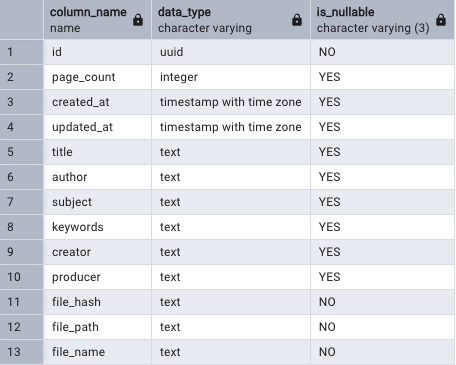
\includegraphics[width=0.7\linewidth]{images/dbtable-documents.png}
    \caption{Documents table description}
    \label{fig:psqlDocumentTableDesc}
\end{figure}


\subsubsection{Table: embeddings}

This table stores the chunk-level data required for semantic search. Each row contains a reference to a document, the original text chunk, its embedding vector, and an embedding hash. During query time, the vector search module returns the top-$K$ most similar vectors based on cosine similarity. The corresponding text chunks are then retrieved from this table using the hash and document ID to form the LLM context (refer to table definition in Fig~\ref{fig:psqlEmbeddingsTable}).

\begin{figure}[H]
    \centering
    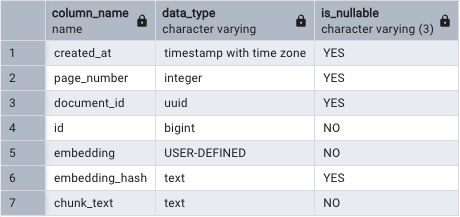
\includegraphics[width=0.7\linewidth]{images/dbtable-embeddings.png}
    \caption{Embeddings table description}
    \label{fig:psqlEmbeddingsTable}
\end{figure}
%----------------------
\subsection{File System: Corpus Directory and Vectordump Files}
\label{subsec:AppDesignModules-FSandVectordump_files}
%----------------------
Vector dump files are binary data structures designed for efficient storage of document embeddings. For each input document, a corresponding vector dump file is created. Each such file contains embedding vectors generated from text chunks along with their corresponding MD5 hashes. This format enables fast similarity search and content verification in document retrieval systems.

%----------------------
\subsubsection{Corpus Directory}
\label{subsec:AppDesignModules-CorpusDir}
%----------------------
The corpus directory serves as the source of truth for the RAG pipeline. It contains the raw documents—primarily PDF files—that are parsed, chunked, and processed by the language model to construct the knowledge base used for information retrieval. 

This project recursively scans the specified corpus directory, identifies all PDF files, and computes their corresponding embeddings and stores them in \textbf{\.vecdump} files.
%----------------------
\subsubsection{Vectordump Files}
\label{subsec:AppDesignModules-Vectordump_FileStructure}
%----------------------
Vector dump files are obtained as a result of the embedding process. After a document is split into chunks, each chunk is processed by the LLM and yields embeddings. Embeddings are higher dimensional representations of the input text, as interpreted by the LLM. 
These embeddings are then stored in a dedicated subdirectory named \textit{\_vecdump}, located within the corpus directory itself. The \textit{\_vecdump} folder houses binary \texttt{.vecdump} files that are later used during the similarity search phase to efficiently retrieve semantically relevant chunks.

The vector dump file follows a sequential binary layout consisting of three main components: a metadata header, followed by embedding data, and finally hash data (as illustrated in Fig~\ref{fig:vectordumpfilestructure}. This structure allows for efficient random access to embeddings while maintaining data integrity through hash verification. Hash is also further used for fetching the corresponding text chunk after similar vectors are obtained for a query.

   \begin{figure}[h]
    \centering
    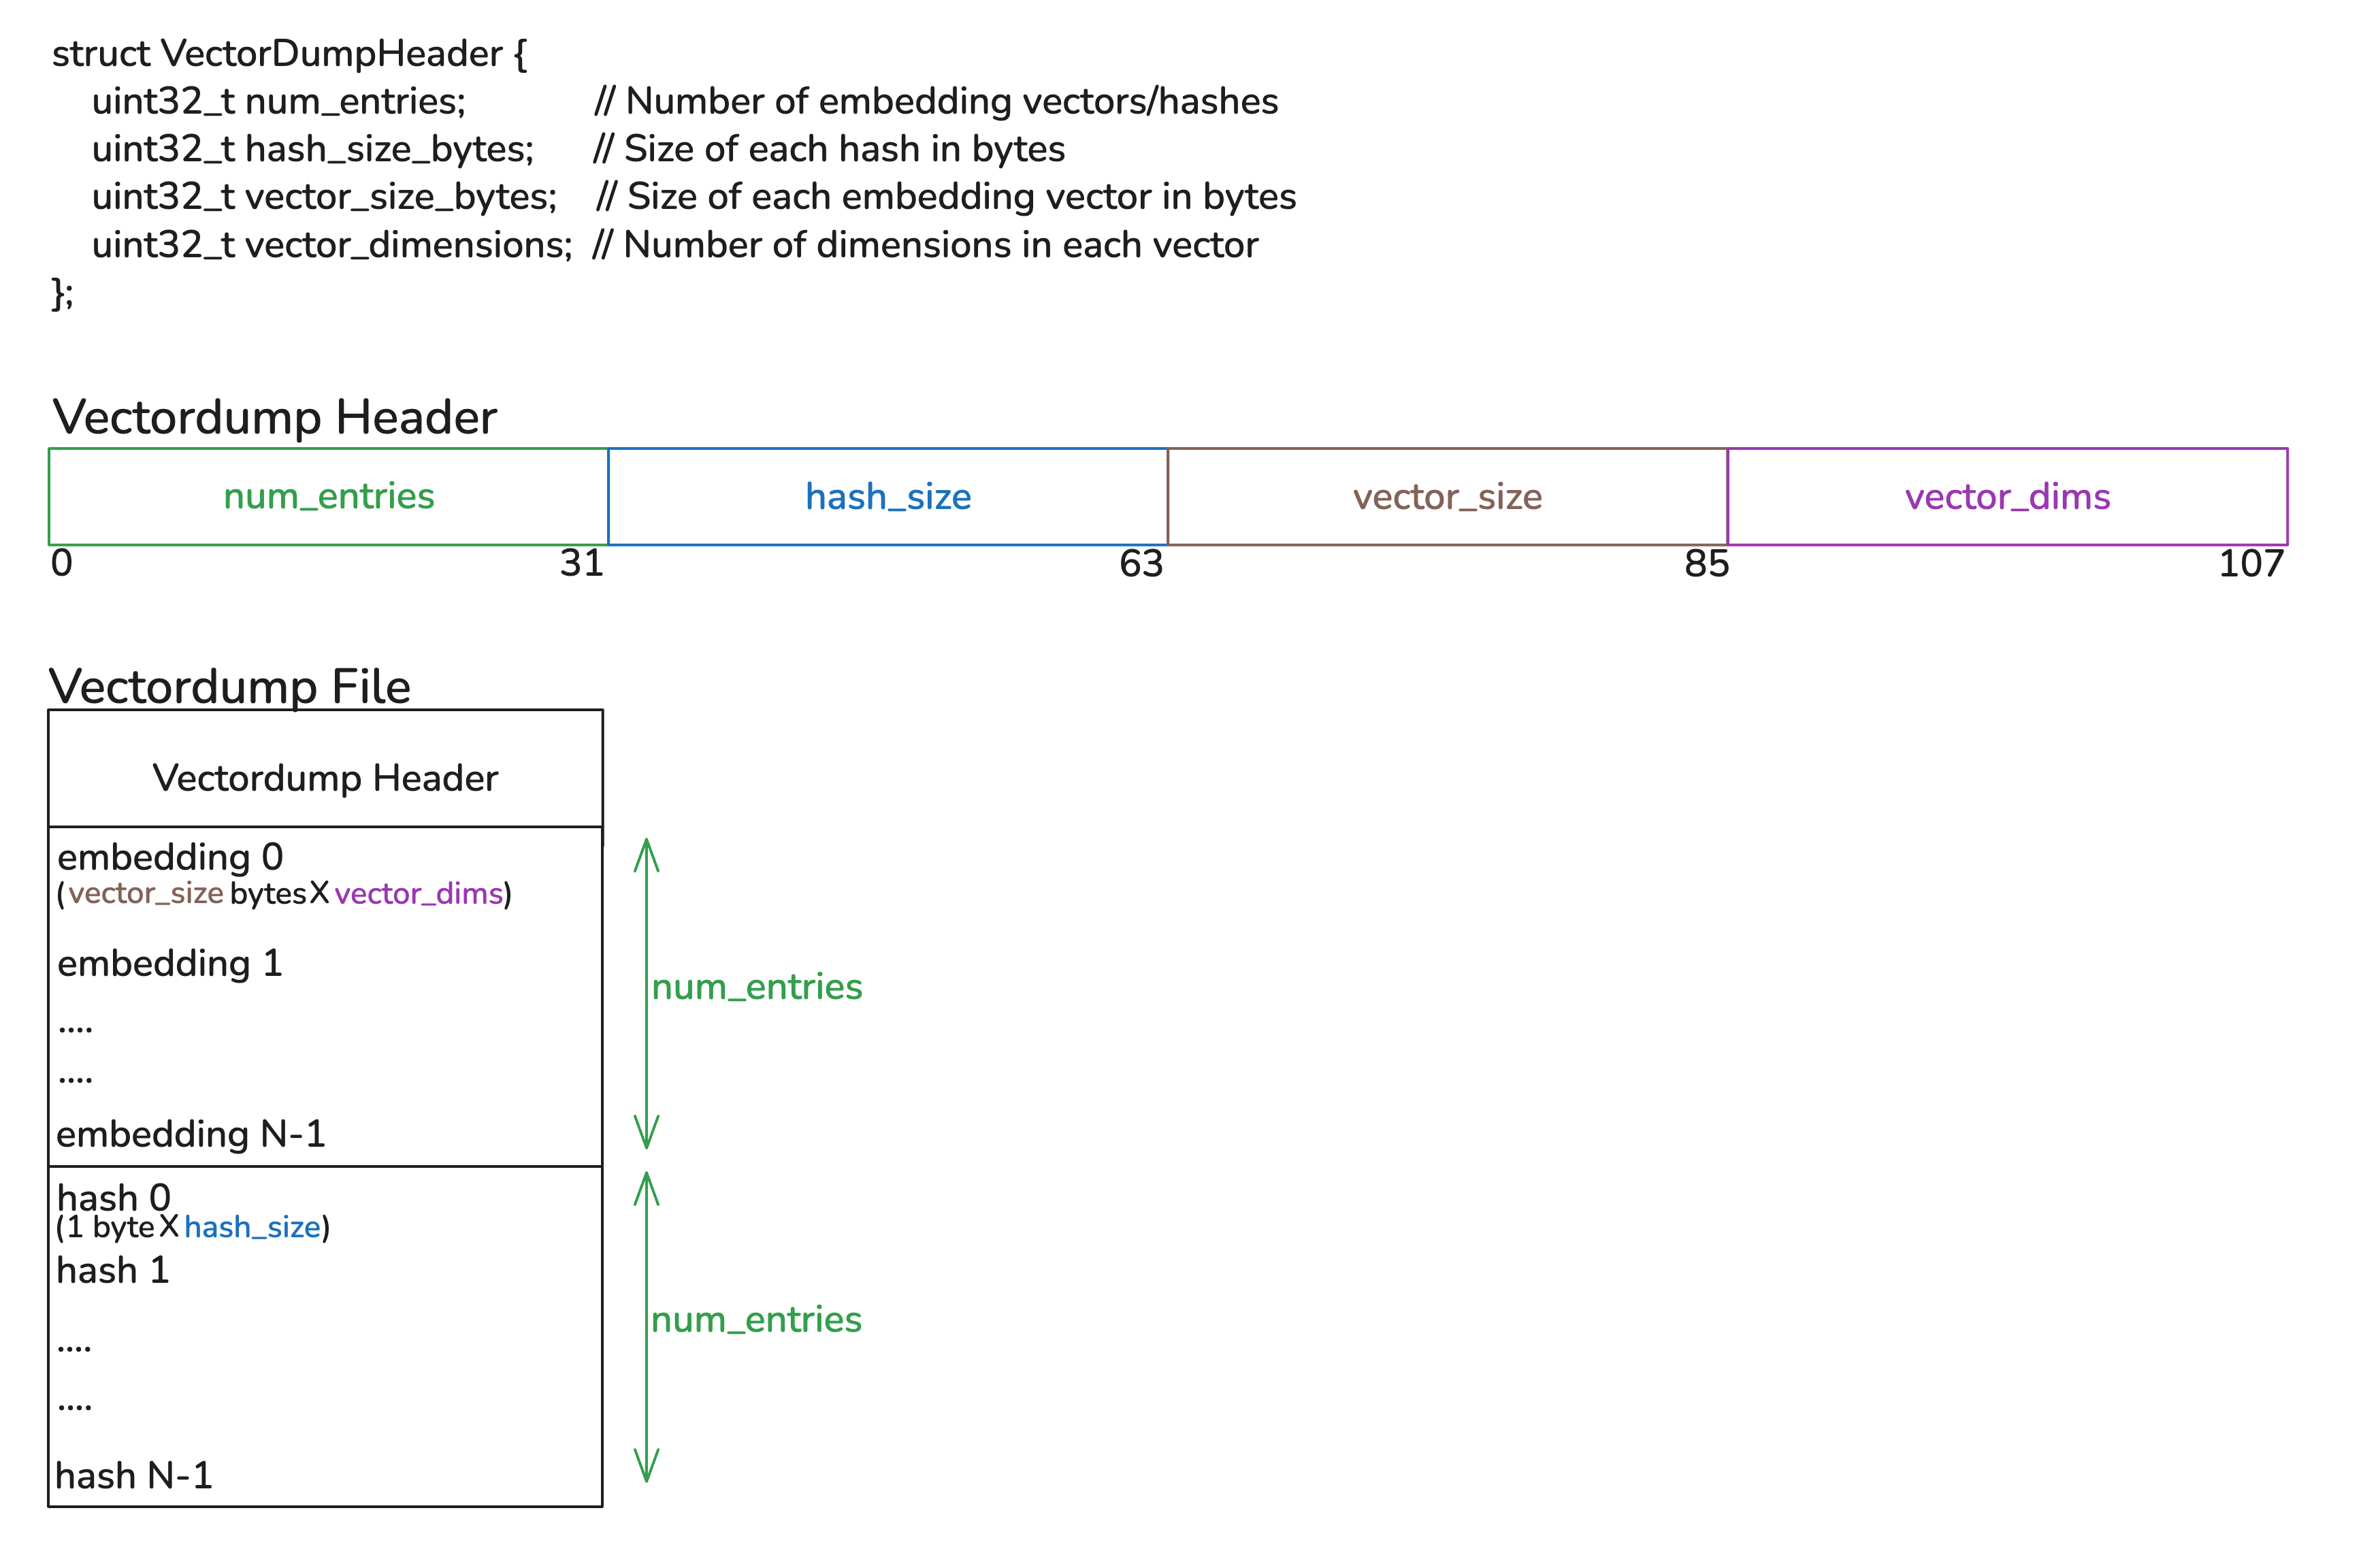
\includegraphics[width=0.9\linewidth]{images/VectorDumpFiles.png}
    \caption{Vector dump file structure}
    \label{fig:vectordumpfilestructure}
\end{figure}

%----------------------
\subsubsection{Vectordump Header}
\label{subsec:AppDesignModules-Vectordump_Header}
%----------------------
In order to process the vector dump file, the header is first read and the necessary information is obtained regarding the data layout in the file. The information is arranged in the layout as illustrated in Figure~\ref{fig:vectordumpfilestructure}. The elements are as follows:
\begin{itemize}
    \item \texttt{num\_entries} - Total number of embedding/hash pairs stored in the file
    \item \texttt{hash\_size\_bytes} - Size of each MD5 hash in bytes (always 16 for standard MD5)
    \item \texttt{vector\_size\_bytes} - Total byte size of each embedding vector
    \item \texttt{vector\_dimensions} - Number of floating-point dimensions per embedding vector
\end{itemize}

The header is read by simply pointing a pointer of type $struct VectorDumpHeader$ to the memory location to which the file is loaded. This helps obtain the necessary information required to access the data sections of the file.

%----------------------
\subsubsection{Data Sections}
\label{subsec:Vectordump_DataSections}
%----------------------
Once the header section is loaded, the data obtained is then used for calculating the memory locations of the embedding and hash arrays.
Pointers are used to access these locations to simulate the structure of an array on top of raw binary data read into the memory. This approach is simple and efficient and prevents needless memory allocations and data copies.

\textbf{Embeddings:} Contains $N$ consecutive embedding vectors, where $N$ = \texttt{num\_entries}. Each vector occupies \texttt{vector\_size\_bytes} and represents a \texttt{vector\_dimensions}-dimensional embedding, stored as 32-bit floating point values. In the current case, we use a 384-dimensional vector embedding.

\textbf{Hashes:} Contains $N$ consecutive MD5 hash values, each exactly 16 bytes. However, the smallest unit of storage is of $uint64_t$ type, i.e., units of 2 bytes. Hence, a 16 byte MD5 hash would have a hash size of 8. The hash at index $i$ corresponds to the MD5 digest of the original text chunk used to generate \texttt{embedding[i]}.


%----------------------
\subsubsection{Data Relationship}
\label{subsec:Vectordump_DataRelationship}
%----------------------

The file maintains strict positional correspondence: for any index $i \in [0, N-1]$, \texttt{embedding[i]} and \texttt{hash[i]} represent the same document chunk. This one-to-one mapping enables efficient lookup operations and integrity verification during retrieval.

The data is used as follows:
\begin{enumerate}[label=\arabic*.]
\item Load the first half of the file in memory using \textbf{mmap} and perform cosine similarity search.
    \item Obtain index of the top $K$ relevant vectors from Cosine similarity module.
    \item Fetch the hash values at the obtained indices.
    \item Query the database for text chunks associated with the hash values.
\end{enumerate}
    
This design allows for prioritized access to necessary data and its direct usage for cosine similarity search with no further processing or data manipulations, allowing for an efficient search through the entire corpus.

%----------------------
\subsection{NPU Accelerated Cosine Similarity}
\label{subsec:AppDesignModules-NpuCosineSim}
%----------------------
The NPU accelerator module (lib-npu\_accelerator) is a specialized component of the TLDR MacOS desktop application that leverages Apple's Neural Processing Unit to perform hardware-accelerated cosine similarity computations as part of the RAG pipeline.
The module construction and usage is a multi-step process involving multiple components. The codebase structure is depicted in Fig~\ref{fig:libnpucodebase} and the workflow in Fig~\ref{fig:libnpuworkflow}.

\subsubsection{Codebase structure}
The codebase for the npu module as seen in Fig~\ref{fig:libnpucodebase} has the following components:
\begin{figure}[h]
    \centering
    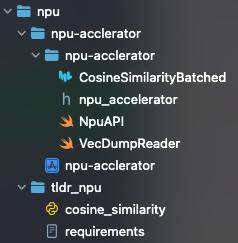
\includegraphics[width=0.4\linewidth]{images/npu-fs.png}
    \caption{lib-npu\_accelerator codebase}
    \label{fig:libnpucodebase}
\end{figure}
\begin{itemize}
    \item \textbf{PyTorch module (\texttt{tldr\_npu}):} Contains PyTorch code to perform batched cosine similarity. This module is used to generate a CoreML model package, which is later utilized by the NPU accelerator for high-performance similarity computation.
    \item \textbf{Swift module (\texttt{npu-accelerator}):} Implements the logic in Swift to read vector dump files and leverage the CoreML cosine similarity model to perform efficient vector similarity search using the Apple Neural Engine (ANE).
\end{itemize}

\subsubsection{Processing Workflow}

\begin{figure}[h]
    \centering
    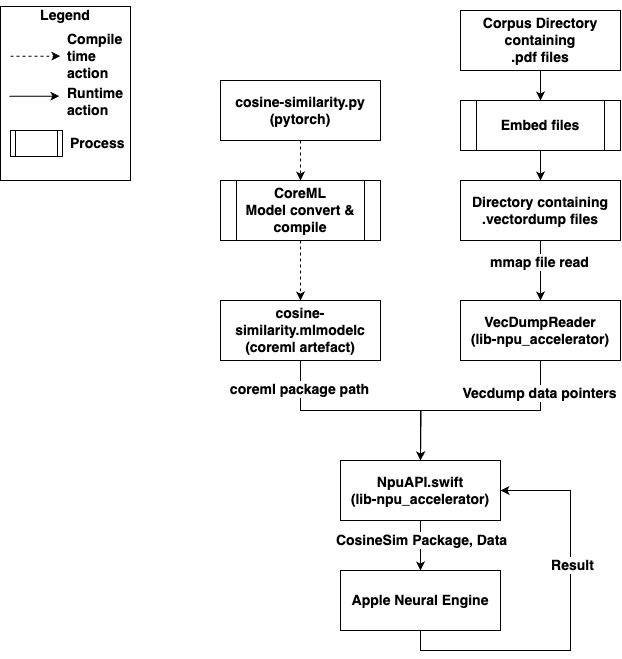
\includegraphics[width=0.7\linewidth]{images/npu-accelerator-module-worklfow.jpg}
    \caption{NPU accelerator module workflow}
    \label{fig:libnpuworkflow}
\end{figure}
The NPU accelerator workflow could be visualized as  dual-pipeline workflow as illustrated in Fig~\ref{fig:libnpuworkflow}. 

\textbf{Phase I - Prepare the components}:
The left pipeline begins with a PyTorch-based cosine-similarity.py implementation that serves as the foundation for similarity computations. This PyTorch model undergoes a CoreML model conversion and compilation process, transforming the original implementation into an optimized CoreML artifact specifically designed for Apple's Neural Engine execution. The compilation step produces the \textit{cosine-similarity.mlmodelc} package, which contains the optimized model ready for hardware acceleration.

The right pipeline operates in parallel, handling document processing and vector storage. Although this portion of the pipeline is  executed by the RAG Backend and is not directly part of the NPU module, it still is a logical component of the NPU module workflow as depicted in Fig~\ref{fig:libnpuworkflow}.

\textbf{Phase II - Perform vector search}:
This phase is triggered at runtime when a user submits a query and the RAG pipeline is activated. The workflow converges at \texttt{NpuAPI.swift}, a Swift-based interface that integrates the CoreML similarity model and the document embeddings obtained via the \texttt{VecDumpReader}.

The \texttt{VecDumpReader} accesses vector dump files using memory-mapped I/O (\texttt{mmap}), exposing the data as raw pointers without intermediate copies. These pointers are passed directly to the \texttt{CosineSimilarityBatched} module, which performs batched cosine similarity computations using Apple's Neural Engine (ANE).

\texttt{NpuAPI} orchestrates this process by coordinating the CoreML model execution and the memory-resident embeddings, enabling efficient hardware-accelerated similarity search. The output consists of similarity scores and embedding hash values, which are used by the RAG system to retrieve the most relevant document chunks for generating a contextually informed response. Furthermore, \texttt{NpuAPI} also serves as a bridge to the C++ layer, exposing these capabilities to the RAG backend for use during the retrieval phase of the RAG pipeline.

Although cosine similarity involves a full scan of the embedded corpus for each query, the system architecture mitigates performance concerns through the following mechanisms:

\begin{itemize}
    \item \textbf{Shared memory-mapped files:} When multiple threads handle different user requests, redundant file reads are avoided because the \texttt{mmap} mechanism loads the file into memory only once.
    
    \item \textbf{Zero-copy access:} Since the data is accessed directly from memory without duplication, there is no overhead for repeated reads. Additionally, the operating system can page the data out to swap memory and page it back in when needed, optimizing memory usage.
    
    \item \textbf{Unified memory architecture:} The Apple M1/M2 SoC’s unified memory architecture enables seamless access between CPU, GPU and NPU, eliminating the need for further data transfers during vector similarity computations.
\end{itemize}

%----------------------
\subsection{llama.cpp}
\label{subsec:AppDesignModules-LLaMaCpp}
%----------------------

The project integrates a customized fork of \texttt{llama.cpp}—a lightweight C++ inference engine for LLaMA and related transformer models—to serve as the core engine for both text generation and embedding extraction. The fork is hosted at \url{https://github.com/manuhg/llama.cpp}, and includes minor modifications that streamline the build process for macOS targets. Specifically, the build scripts were stripped down to produce a static library using the \texttt{ggml} Metal backend, optimized for Apple Silicon devices.  The result is a single, portable C++ static library named \texttt{libllama.a} which is then statically linked with the RAG backend (\texttt{lib-tldr.a}).

The core functionalities such as tokenization, decoding, and sampling are accessed through the public APIs exposed in \texttt{llama.h} and \texttt{ggml.h}. Two primary components—\texttt{LLmChat} and \texttt{LLmEmbedding}—are built around workflows inspired by \textttt{simple.cpp}~\cite{llama_simple} \texttt{server.cpp}~\cite{llama_server} and \texttt{embedding.cpp}~\cite{llama_embedding} from the upstream \texttt{llama.cpp}~\cite{llamacpp} project. 

Further, to improve the performance, \texttt{OpenMP} support was added for parallelizing the tokenization and batch decoding steps. This optimization ensures efficient utilization of CPU cores, resulting in faster preprocessing and inference, particularly during multi-threaded interactions.

The \texttt{llama.cpp} is hence directly integrated into the RAG backend at compile time. This enables the application to perform in-memory LLM inference by directly invoking components of \texttt{llama.cpp}, without relying on any external dependencies or background processes for this core functionality.
%----------------------
%----------------------
\section{Application Workflow}
\label{sec:AppWorkflow}
%----------------------

%----------------------
\subsection{Workflow Overview}
\label{subsec:AppDesignWorkflow-Overview}
%----------------------

\begin{figure}[H]
    \centering
    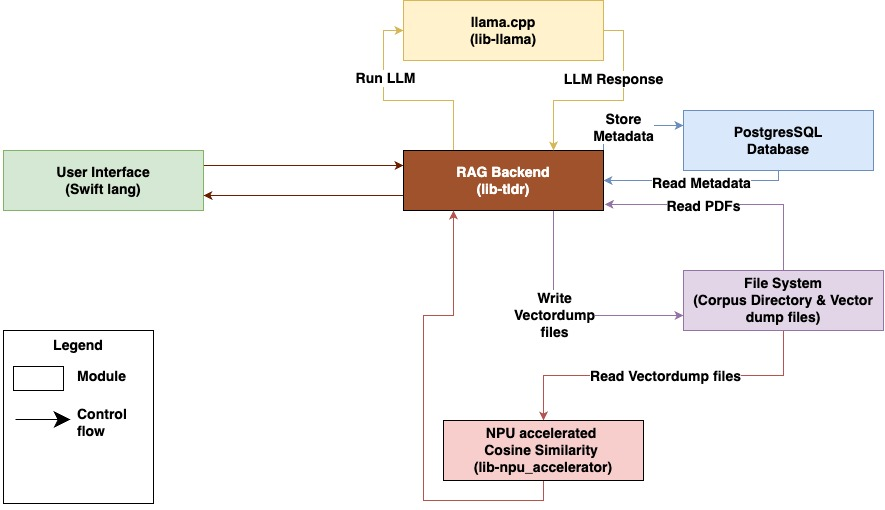
\includegraphics[width=1.0\linewidth]{images/tldr-app-module-interactions.jpg}
    \caption{TLDR application module interactions}
    \label{fig:tldrmodulesinteraction}
\end{figure}

Figure~\ref{fig:tldrmodulesinteraction} illustrates the high-level architecture of the TLDR application, highlighting its modular design and control flow between components.

At the center is the \textbf{RAG Backend} (\texttt{lib-tldr}), which serves as the core orchestrator. It interfaces with several specialized modules to perform retrieval-augmented generation.

\begin{itemize}
    \item The \textbf{User Interface}, interacts with the RAG backend to initiate queries and display responses to the user.
    
    \item \textbf{llama.cpp} (\texttt{lib-llama}) is linked as a static library and provides language model functionality. The backend calls it for both text generation and embedding, receiving outputs directly in memory.
    
    \item \textbf{PostgreSQL Database} is used to store and retrieve document metadata and precomputed embeddings. The RAG backend communicates with it to persist and query structured data including document metadata and text chunks for embeddings.
    
    \item The \textbf{File System} acts as the persistent store for documents and vector dumps. The backend reads PDF files for embedding and writes embedding outputs into binary vector dump files.
    
    \item \textbf{NPU-Accelerated Cosine Similarity} (\texttt{lib-npu\_accelerator}) reads the vector dump files through memory-mapped I/O and executes similarity search using a CoreML model on Apple's Neural Engine (ANE).
\end{itemize}

This modular architecture allows each component to focus on a specific responsibility while maintaining efficient communication with the core backend. All dependencies are statically compiled or locally integrated, ensuring portability and performance.


%----------------------
\subsection{RAG Pipeline Workflow}
\label{subsec:RAGWorkflow}
%----------------------
The workflow of the modules of the system and the RAG pipeline can be divided into 3 logical phases. 
\begin{itemize}
    \item System Initialization: Initializes the resources required by the system.
    \item Embedding Phase: Generate embeddings for documents in the source corpus.
    \item Retrieval and Generation Phase: Leverage embedded documents to retrieve information relevant to a query made by the user and generate a response using the LLM.
\end{itemize}
The following sections show a detailed breakdown of these phases.

%----------------------
\subsubsection{System Initialization}
\label{subsec:AppDesignWorkflow-SystemInitialization}
%----------------------

\begin{figure}[H]
    \centering
    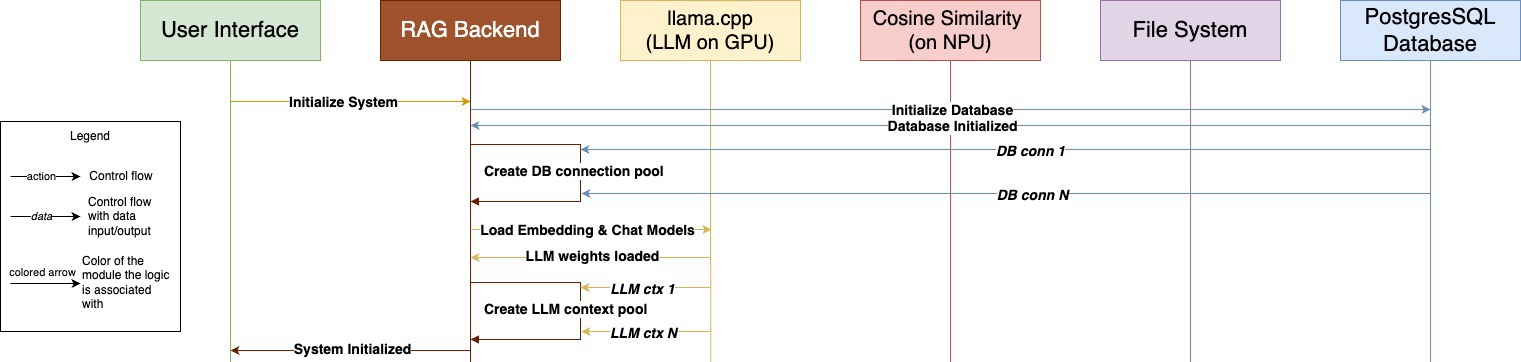
\includegraphics[width=1.0\linewidth]{images/tldr-app-worklfow-pt1.jpg}
    \caption{RAG Output evaluation metrics ~\cite{cardenas2023rag}}
    \label{fig:autoregressive_decoding}
\end{figure}


The initialization phase sets up the backend infrastructure and prepares the application for use. This includes:

\begin{itemize}
    \item The user launches the application, triggering the backend.
    \item The \textbf{RAG Backend} initializes a connection pool to the \textbf{PostgreSQL Database}.
    \item The LLM weights and context pools are loaded via \texttt{llama.cpp}, enabling multi-threaded inference.
    \item Cosine similarity routines are prepared via the \textbf{NPU accelerator} module.
    \item System status is communicated back to the \textbf{User Interface}, indicating readiness.
\end{itemize}


%----------------------
\subsubsection{Embedding the Corpus}
\label{subsec:AppDesignWorkflow-EmbeddingCorpus}
%----------------------

\begin{figure}[H]
    \centering
    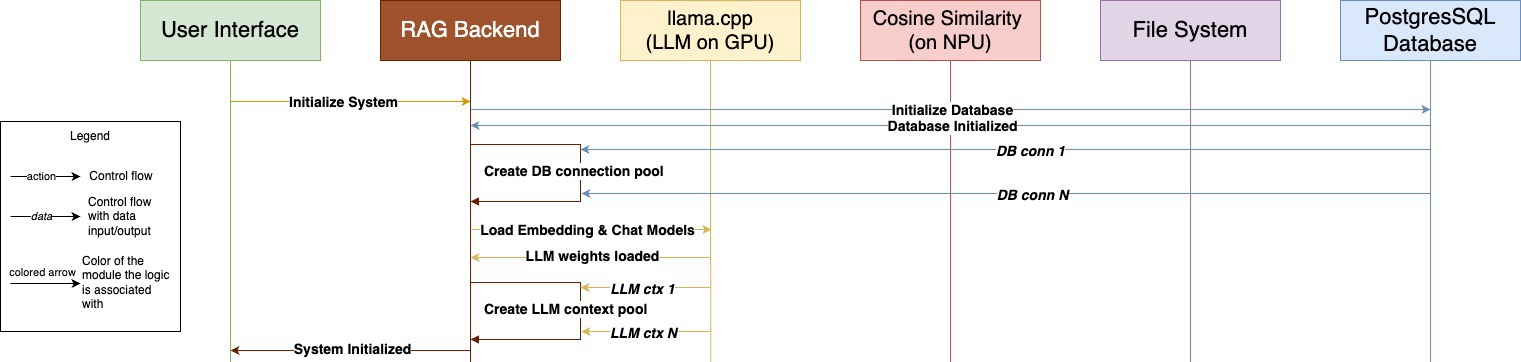
\includegraphics[width=1.0\linewidth]{images/tldr-app-worklfow-pt1.jpg}
    \caption{RAG Output evaluation metrics ~\cite{cardenas2023rag}}
    \label{fig:autoregressive_decoding}
\end{figure}

When a user selects a directory to embed the following actions take place:
\begin{itemize}
    \item The \textbf{RAG Backend} scans the specified directory for documents using the File System.
    \item Each document is loaded, chunked, and converted to embeddings using a pre-defined embedder.
    \item Embeddings, text chunks, and associated metadata are inserted into the \textbf{PostgreSQL Database}.
    \item In parallel, the backend also writes a vector dump file to the \textbf{File System}, which stores the hash of each vector for quick access.
\end{itemize}
This dual-storage mechanism (DB + mmap vector cache) allows fast retrieval during inference while maintaining queryable metadata.

%----------------------
\subsubsection{Performing RAG}
\label{subsec:AppDesignWorkflow-PerformingRAG}
%----------------------
\begin{figure}[H]
    \centering
    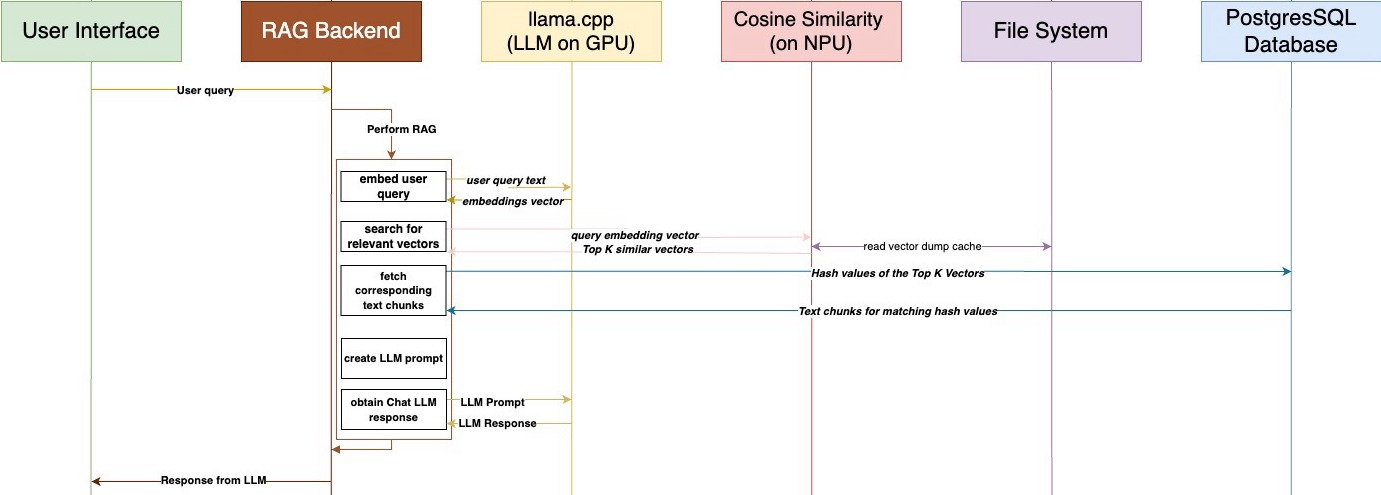
\includegraphics[width=1.0\linewidth]{images/tldr-app-worklfow-pt3.jpg}
    \caption{RAG Output evaluation metrics ~\cite{cardenas2023rag}}
    \label{fig:autoregressive_decoding}
\end{figure}

Once the corpus is embedded, the system is ready to answer user's queries. When the user proceeds to inquire the system, the following steps are executed:

\begin{itemize}
    \item The user query is embedded using the same embedding model.
    \item The embedded query vector is sent to the \textbf{Cosine Similarity} module running on the NPU.
    \item A top-$k$ similarity search is performed against memory-mapped vector files using the NPU, returning hash values of the best matches.
    \item These hashes are used to retrieve the corresponding text chunks from the \textbf{PostgreSQL Database}.
    \item A prompt is constructed and sent to the \textbf{LLM} via \texttt{llama.cpp}.
    \item The generated response is sent back to the \textbf{User Interface}.
\end{itemize}


With these steps, the TLDR project is able to perform retrieval augmented generation on documents present in the user's device, without requring any external resources or internet access.
